\documentclass[10pt,twocolumn,a4paper]{article}
\usepackage[a4paper,top=0.75in,bottom=0.85in,left=0.68in,right=0.68in,columnsep=0.25in]{geometry}
\usepackage{mathptmx}
\usepackage[T1]{fontenc}
\usepackage[utf8]{inputenc}
\usepackage{graphicx,amsmath,amssymb,booktabs,array,titlesec,caption,cite}
\usepackage[hidelinks]{hyperref}
\usepackage{url}
\renewcommand{\thesection}{\Roman{section}}
\renewcommand{\thesubsection}{\Alph{subsection}}
\titleformat{\section}[block]{\centering\normalsize\scshape}{\thesection.}{0.5em}{}
\titleformat{\subsection}[block]{\normalsize\itshape}{\thesubsection.}{0.5em}{}
\titlespacing*{\section}{0pt}{1.5ex}{1ex}
\captionsetup{font=small,labelsep=period}
\setlength{\parindent}{1em}
\setlength{\emergencystretch}{1.5em}
\newcommand{\regRMSE}{667,507}
\newcommand{\regMAE}{56,568}
\newcommand{\regRsq}{0.104}
\newcommand{\regMedAPE}{8.74}
\newcommand{\regWithin}{77.4}
\newcommand{\treeFone}{0.9218}
\newcommand{\treeAUC}{0.9670}
\newcommand{\linearFone}{0.9037}
\newcommand{\rffFone}{0.9088}
\newcommand{\treeValFone}{0.9253}
\newcommand{\rffValFone}{0.9136}
\newcommand{\linearValFone}{0.9095}
\newcommand{\sseShare}{98.8}
\newcommand{\testMax}{60,000,000}
\newcommand{\nearError}{28.0}
\newcommand{\farError}{5.2}
\newcommand{\cvMedAPE}{9.22}
\newcommand{\cvMedAPEsd}{0.05}
\newcommand{\areaImportance}{40.4}
\newcommand{\logAreaWeight}{3.158}
\newcommand{\rawAreaWeight}{-0.477}
\newcommand{\authorline}{MLE-AI-201 Course Project}
\newcommand{\repositoryline}{Repository URL has not been supplied; reproducible source is included in the companion project package.}

\begin{document}
\twocolumn[
\begin{@twocolumnfalse}
\begin{center}
{\LARGE\bfseries Residential Asking-Price Prediction\\with NumPy Decision Trees and Pegasos SVMs\par}
\vspace{0.8em}
{\large\authorline\par}
\vspace{0.3em}
{\itshape AI Academy / National AI Center --- Final Project V3\par}
\vspace{0.7em}
\end{center}
\begin{quote}\small
\noindent\textbf{\textit{Abstract---}}
This project studies residential asking prices and a derived premium-price classification task using a bina.az listing snapshot. After retaining the latest snapshot of each listing, the declared residential scope contains 58,452 rows. Conservative duplicate-property groups are kept disjoint across training, validation and test. All feature statistics, geographical centres and the premium threshold are learned from training data. We implement exact-split decision trees, a mini-batch Pegasos solver and random Fourier features directly in NumPy. Matched scikit-learn estimators provide comparison baselines. Validation selects separate spatial log-price trees for apartments and detached houses, and an entropy tree for classification. On the 8,724-row test subset, the own regressor obtains RMSE \regRMSE{} AZN, MAE \regMAE{} AZN and median absolute percentage error \regMedAPE\%. The own classifier achieves F1 \treeFone{} and ROC AUC \treeAUC; linear and nonlinear SVMs remain required, separately evaluated models. Five-fold grouped checks reveal severe squared-error instability caused by an unverified extreme training price. We report this limitation without removing evaluation rows. \repositoryline

\vspace{0.4em}
\noindent\textbf{\textit{Index Terms---}}decision tree, Pegasos, random Fourier features, residential listings, grouped evaluation.
\end{quote}
\vspace{0.4em}
\end{@twocolumnfalse}
]

\section{Problem and contributions}
Task A predicts a listing's price in AZN. Task B predicts whether that price exceeds the residential training median. These are distinct tasks: classification F1 is not a percentage accuracy measure for price estimation. The project emphasizes correct algorithm implementations and defensible experiments, rather than a promised production valuation.

The core contributions are a NumPy tree supporting regression and classification, a NumPy linear hinge-loss solver with a required nonlinear extension, a leakage-controlled data pipeline, and matched library comparisons. An additional train-only geographical clustering analysis supports interpretation. Commercial property, offices, land and garages are outside the declared scope; new apartments, old apartments and detached/garden houses remain. This choice was made during validation work and limits the population to which the results apply.

\section{Data and experimental population}
\subsection{Cleaning and provenance}
The supplied \texttt{house\_sale.csv} contains 100,775 rows and 51 columns. Scrape timestamps span 5 October--19 November 2024. These are advertised prices, not verified transactions or current 2026 market values. The source is the course's bina.az sale dataset~\cite{data}.

Both currency fields are verified as AZN. The pipeline keeps the latest detail scrape for each canonical listing URL, with source-row order resolving timestamp ties. Removing 36,321 older snapshots leaves 64,454 listings; 58,452 belong to the declared residential categories. Thirteen disagreements between \texttt{price} and \texttt{total\_price} are recorded without substituting the target.

Explicit area units are converted to square metres; one sot equals 100 square metres. Invalid numeric values become missing. Floor and total-floor values are parsed separately, then floor ratio and area per room are derived. One implausible coordinate pair is set missing. Missing mortgage information remains unknown rather than being interpreted as no mortgage.

Training data include a 600,000,000 AZN price for a 200 m$^2$ listing and unusually low prices. Such values need source review. The main comparison retains them because a statistically extreme value is not proof of an erroneous label. Earlier training-only sensitivity work is documented in the development history; it does not remove test observations or silently repair final targets.

\subsection{Features and leakage prevention}
The base representation uses ten numeric features: area, land area, rooms, floor, total floors, floor ratio, latitude, longitude, log area and area per room. Six categorical fields represent city, location, category, repair, bill of sale and mortgage. Numeric imputation medians, missingness flags, categorical vocabularies and rare-category rules are fitted only on the current training fold. Categories occurring fewer than 20 times share a rare bucket; unseen and missing values have distinct buckets. The final classifier input has 141 columns.

An explicit feature allowlist excludes \texttt{unit\_price}, \texttt{total\_price}, price-derived predictors, owner/shop identifiers, raw addresses, URLs and free text. Normalized descriptions and identifiers are used only to construct duplicate groups and audit records. They never enter the estimators.

\subsection{Split and task definition}
Potential duplicate-property listings share a group if a sufficiently long normalized description and selected physical/location fields agree. The signature excludes price. This is a conservative proxy, not a verified property ID. It may miss reworded listings or group unrelated records.

Seed 42 first chooses approximately 70\% of full-data groups without consulting price. The remaining groups are split into validation and test strata using the original full-training median (210,000 AZN). Residential filtering preserves these established memberships. The final residential premium definition is strictly \textbf{price $>$ 207,000 AZN}, the median of its training subset. Earlier full-scope classification results therefore are not directly comparable with the final task.

\begin{table}[t]\centering\small
\caption{Final residential split; property groups do not overlap.}
\begin{tabular}{@{}lrrr@{}}
\toprule
Subset & Rows & Groups & Premium \\
\midrule
Train & 40,932 & 40,422 & 49.91\% \\
Validation & 8,796 & 8,692 & 51.05\% \\
Test & 8,724 & 8,622 & 50.84\% \\
\bottomrule
\end{tabular}

\end{table}
The training, validation and test subsets contain 40,932, 8,796 and 8,724 rows. No median or preprocessing parameter is estimated from validation or test. Evaluation retains every residential row in its assigned subset.

\begin{figure}[t]\centering
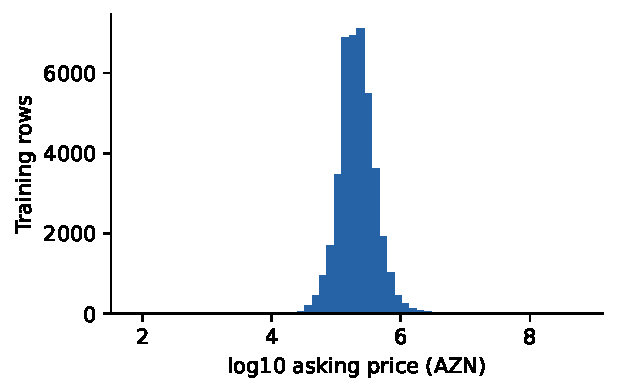
\includegraphics[width=\columnwidth]{figures/report_eda.pdf}
\caption{Training price distribution on a log scale. Extreme records remain in the data; other EDA figures accompany the notebook.}
\end{figure}

\section{Algorithms}
\subsection{Decision trees}
At each node, the own implementation sorts each numeric feature and evaluates the midpoint between every pair of distinct adjacent values. Prefix class counts or centred squared-error sums make the search efficient. Classification supports Gini impurity and base-two entropy; regression minimizes MSE. Candidate splits maximize the parent impurity reduction after weighting child impurities by sample count.

Recursive growth implements maximum depth, minimum split size, minimum leaf size and minimum global impurity decrease. The latter weights local improvement by node size divided by root size. Zero-gain splits are permitted, allowing an XOR sanity case to split before becoming informative. Regression leaves predict the mean of their training targets. Classification leaves predict the majority class and return empirical class frequencies as probabilities. Feature importance sums weighted impurity decreases and normalizes them.

The selected regressor fits log price. A category-based router trains separate apartment and detached-house trees, each with depth 16 and minimum leaf size 5. Predictions are exponentiated, yielding a geometric-mean leaf price rather than an unbiased arithmetic-mean estimate. This stabilizes large targets but can underpredict the upper price tail.

Spatial features are great-circle distances to an Old City reference coordinate~\cite{unesco} and to twelve train-fitted geographical centres. Centres use a seeded NumPy k-means procedure on a local distance projection. They are data summaries, not metro stations or official districts. The classifier selected entropy, depth 16 and minimum leaf size 10.

\subsection{Linear Pegasos}
For labels $y_i\in\{-1,+1\}$, the implemented objective is
\begin{equation}
J(w,b)=\frac{\lambda}{2}\|w\|^2+
\frac1n\sum_i\max(0,1-y_i(w^\top x_i+b)).
\end{equation}
Following the primal subgradient approach~\cite{pegasos}, each epoch shuffles training rows and processes mini-batches of at most 256 rows. With active set $A=\{i:y_i(w^\top x_i+b)<1\}$ in batch $B$,
\begin{align}
\eta_t&=(\lambda t)^{-1},\\
w'&=(1-\eta_t\lambda)w+\frac{\eta_t}{|B|}\sum_{i\in A}y_i x_i,\\
b'&=b+\frac{\eta_t}{|B|}\sum_{i\in A}y_i .
\end{align}
The bias is separate and unregularized. The vector $w'$ is projected onto the ball of radius $1/\sqrt{\lambda}$. Final coefficients average iterates from the second half of training. Standardization uses current-training means and population standard deviations; constant columns use scale one. The selected linear model uses $\lambda=10^{-3}$ and 120 epochs. Constant and inverse-square-root schedules are diagnostic alternatives, not described as Pegasos.

The recorded objective need not decrease at every stochastic step. We show its trajectory and final value, not a claim of monotonic convergence or an exact optimum. Training points with signed margin at most one form the reported margin-violator/support candidate set; this is not a dual solver's exact nonzero-coefficient support set.

\subsection{Nonlinear extension}
Own random Fourier features approximate an RBF kernel~\cite{rff}:
\begin{equation}
\begin{aligned}
z(x)&=\sqrt{2/m}\cos(xW+c),\\
W_{jk}&\sim\mathcal N(0,2\gamma),\quad c_k\sim U(0,2\pi).
\end{aligned}
\end{equation}
The same own linear solver learns in this feature space. Validation selects $\gamma=0.005$, $m=2,048$, $\lambda=10^{-5}$ and 120 epochs. This avoids storing an $n\times n$ kernel matrix but adds mapping cost and a dense $n\times m$ array (about 671 MB for the final training subset in float64). Margin widths are in the respective standardized or Fourier feature space and should not be compared as physical price distances.

\section{Experiments and verification}
\subsection{Selection protocol}
Seven residential regression configurations compare depth/leaf settings, spatial features and category routing. Classification compares Gini versus entropy, depths 8/12/16, and leaf sizes 5/10. The SVM search tests three linear regularization values and a $3\times3$ bandwidth/regularization grid with 1,024 features. Two bounded follow-up trials increase the best RFF configuration to 2,048 features and then 120 epochs. Linear epoch and schedule diagnostics are included. Short pilot runs preceded the recorded final search.

Validation RMSE selects the regressor; positive-class F1 selects each classifier and the overall classification winner. The final validation F1 values are \treeValFone{} (tree), \linearValFone{} (linear SVM) and \rffValFone{} (RFF SVM). The frozen configuration, dataset fingerprint and timestamp are saved before test scoring. Final models fit only original training rows; validation is not merged back into training.

\begin{figure}[t]\centering
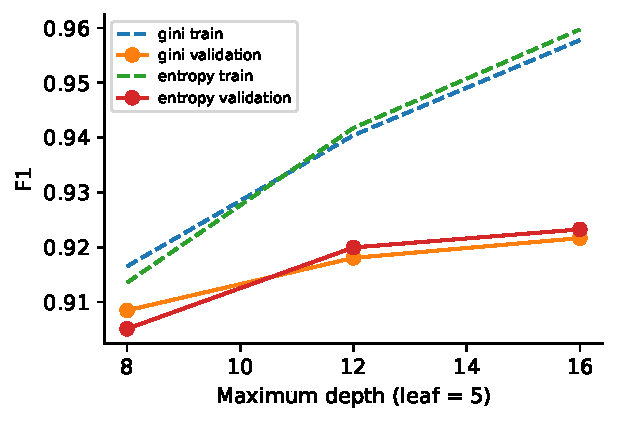
\includegraphics[width=\columnwidth]{figures/report_tuning.pdf}
\caption{Tree capacity diagnostic. Training F1 rises faster than validation F1. SVM tuning and margin figures accompany the notebook.}
\end{figure}

\subsection{Matched baselines and tests}
The tree baselines use the same features, target transform, category routing, criterion, depth and minimum leaf size. Exact predictions can differ because equal-gain choices, random feature order and floating-point thresholds differ. Toy cases with a unique best split agree with scikit-learn.

The SVM baselines use \texttt{SGDClassifier} with hinge loss, L2 penalty and matching $\alpha=\lambda$~\cite{sklearn}. Scaling is inside a fitted \texttt{Pipeline}; the RFF baseline shares the same own mapper to isolate solver differences. Both use 120 epochs, but sklearn performs sample-wise updates with its optimal schedule and averaging, while the own solver uses projected mini-batches and suffix averaging. These are matched objectives, not identical optimization paths. Neither core module imports sklearn.

The automated suite tests split disjointness, train-only preprocessing, all tree stopping rules, exact toy splits, objective arithmetic, a projected Pegasos update, deterministic refits, label mapping, separable-data agreement with sklearn and nonlinear XOR recovery. RFF inner products are also compared with their RBF targets. Tests are accompanied by an executed final notebook.

\subsection{Metrics and uncertainty}
Regression reports RMSE and MAE in AZN, dimensionless $R^2$, median absolute percentage error (MedAPE) and coverage within 20\%. Classification reports precision, recall, F1, ROC AUC, average precision (AP) and a confusion matrix. AP is the non-interpolated precision--recall summary used here.

Five-fold shuffled GroupKFold on the original training subset refits every encoder, spatial centre and model. The premium definition remains fixed at 207,000 AZN as the declared task label. CV evaluates already selected configurations; it is a stability analysis, not nested model selection. Fold mean and sample standard deviation are shown separately from the final held-out test, and are not confidence intervals for that test.

\section{Results}
\begin{table*}[t]\centering
\caption{Held-out test regression, all 8,724 residential rows. RMSE and MAE are in AZN. Lower error is better.}
\begin{tabular}{@{}lrrrr@{}}
\toprule
Model & RMSE & MAE & $R^2$ & MedAPE \\
\midrule
Training median & 708,732 & 140,927 & -0.010 & 39.12\% \\
Own spatial trees & 667,507 & 56,568 & 0.104 & 8.74\% \\
sklearn spatial trees & 666,545 & 56,592 & 0.106 & 8.71\% \\
\bottomrule
\end{tabular}

\end{table*}
\begin{table*}[t]\centering
\caption{Held-out test classification. Positive class is price $>$ 207,000 AZN. Higher is better.}
\begin{tabular}{@{}lrrrrr@{}}
\toprule
Model & Precision & Recall & F1 & ROC AUC & AP \\
\midrule
Training majority & 0.000 & 0.000 & 0.000 & 0.500 & 0.508 \\
Own tree & 0.929 & 0.914 & 0.922 & 0.967 & 0.960 \\
sklearn tree & 0.931 & 0.914 & 0.922 & 0.968 & 0.961 \\
Own linear SVM & 0.906 & 0.902 & 0.904 & 0.967 & 0.967 \\
SGD linear & 0.906 & 0.900 & 0.903 & 0.967 & 0.967 \\
Own RFF SVM & 0.913 & 0.905 & 0.909 & 0.972 & 0.972 \\
SGD + same RFF & 0.915 & 0.905 & 0.910 & 0.972 & 0.972 \\
\bottomrule
\end{tabular}

\end{table*}
\begin{table*}[t]\centering\small
\caption{Separate five-fold grouped training checks (mean $\pm$ sample SD). These are not repeated test-set measurements.}
\begin{tabular}{@{}lrr@{}}
\toprule
Model & RMSE mean $\pm$ SD & F1 mean $\pm$ SD \\
\midrule
Own linear SVM & -- & 0.9061 $\pm$ 0.0038 \\
Own RFF SVM & -- & 0.9111 $\pm$ 0.0023 \\
Own tree & -- & 0.9183 $\pm$ 0.0023 \\
Own spatial trees & 1,431,886 $\pm$ 2,904,141 & -- \\
SGD linear & -- & 0.9061 $\pm$ 0.0043 \\
SGD + same RFF & -- & 0.9114 $\pm$ 0.0024 \\
sklearn tree & -- & 0.9185 $\pm$ 0.0024 \\
sklearn spatial trees & 1,434,084 $\pm$ 2,902,905 & -- \\
\bottomrule
\end{tabular}

\end{table*}

The validation-selected price model achieves test $R^2=\regRsq$ and MedAPE \regMedAPE\%; \regWithin\% of test rows have absolute percentage error at most 20\%. This is useful typical-case performance but does not imply uniformly reliable prices. The own classifier obtains test F1 \treeFone. The linear and RFF variants obtain \linearFone{} and \rffFone, respectively. The required SVM models remain part of the submission even though the tree won validation selection.

\begin{figure}[t]\centering
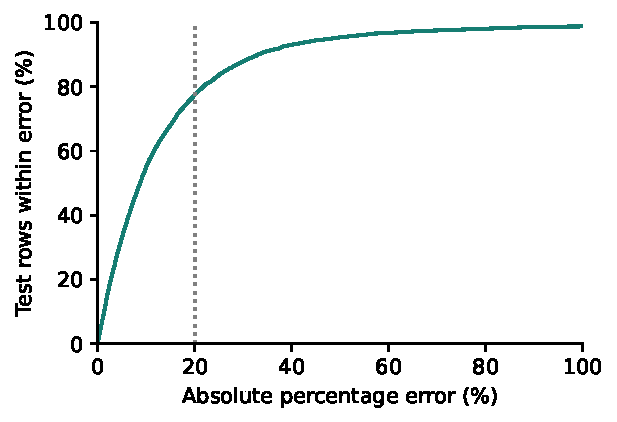
\includegraphics[width=\columnwidth]{figures/report_regression.pdf}
\caption{Relative-error coverage on all test rows, showing error thresholds up to 100\%.}
\end{figure}
\begin{figure}[t]\centering
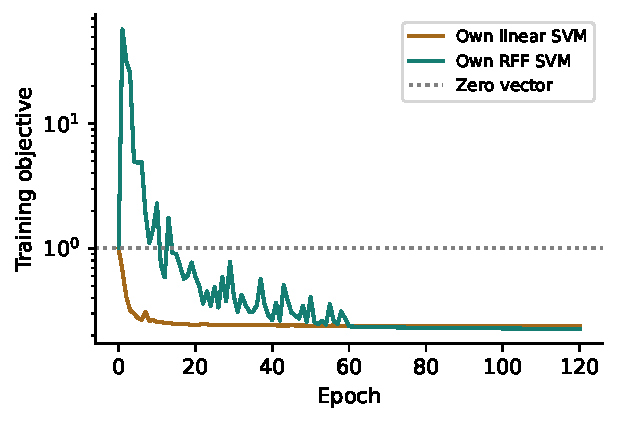
\includegraphics[width=\columnwidth]{figures/report_svm_objective.pdf}
\caption{Training objective using suffix averages once available, and raw iterates beforehand. Stochastic updates need not decrease monotonically.}
\end{figure}
\begin{table}[t]\centering\small
\caption{Final training SVM diagnostics. Margin set means signed margin $\leq1$.}
\begin{tabular}{@{}lrrrr@{}}
\toprule
Model & $J$ & $\|w\|$ & $2/\|w\|$ & Margin set \\
\midrule
Own linear SVM & 0.2380 & 3.575 & 0.559 & 24.2\% \\
Own RFF SVM & 0.2261 & 60.817 & 0.033 & 21.2\% \\
\bottomrule
\end{tabular}

\end{table}
\begin{table}[t]\centering\small
\caption{Own tree classifier's held-out test confusion matrix.}
\begin{tabular}{lrr}
Actual / predicted & Standard & Premium \\
\hline
Standard & 3981 & 308 \\
Premium & 380 & 4055 \\
\end{tabular}

\end{table}
\begin{figure}[t]\centering
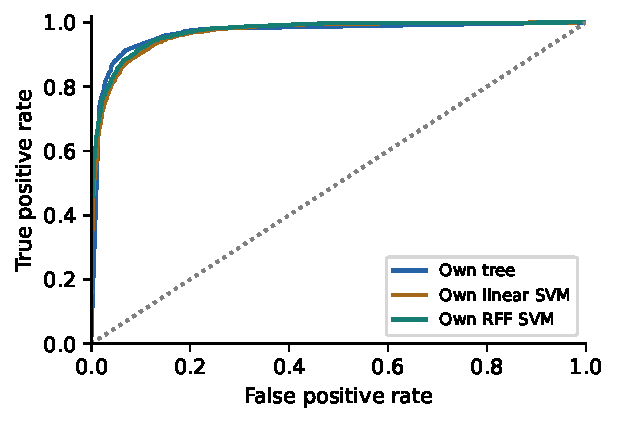
\includegraphics[width=\columnwidth]{figures/report_roc.pdf}
\caption{Test ROC curves; complete precision--recall curves are supplied with the notebook.}
\end{figure}

\section{Error analysis and computational cost}
\subsection{Price-label risk}
The highest 1\% of squared errors account for \sseShare\% of total test squared error. The largest test price is \testMax{} AZN. This concentration explains why RMSE and typical relative error tell different stories. All rows remain in the headline evaluation.

The five-fold check places the 600 million AZN training record in an evaluation fold once, causing extreme RMSE dispersion. The own regressor's fold MedAPE is much more stable at \cvMedAPE$\pm$\cvMedAPEsd\%. This disagreement is evidence of label-quality risk, not justification for hiding the high-error fold. The project cannot claim verified real-world accuracy until the suspicious records are audited against trustworthy sources.

\begin{table}[t]\centering\small
\caption{Own price model's test error by property category.}
\begin{tabular}{@{}lrrr@{}}
\toprule
Category & n & MAE (AZN) & MedAPE \\
\midrule
Detached / garden & 1,451 & 123,771 & 19.80\% \\
Old apartments & 1,859 & 20,849 & 7.97\% \\
New apartments & 5,414 & 50,821 & 7.50\% \\
\bottomrule
\end{tabular}

\end{table}
\begin{figure}[t]\centering
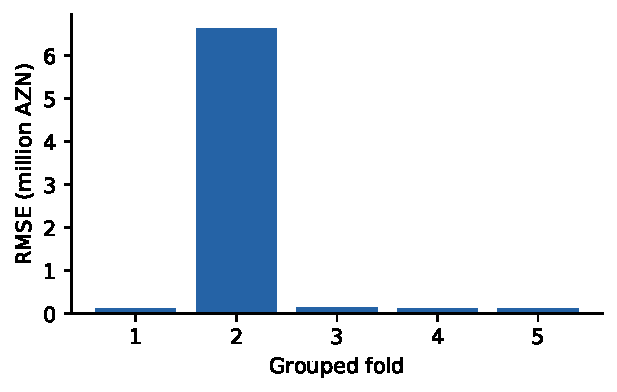
\includegraphics[width=\columnwidth]{figures/report_cv.pdf}
\caption{Grouped-fold RMSE is dominated by the fold containing an unverified extreme price.}
\end{figure}

\subsection{Classification and interpretation}
For the selected classifier, test error is \nearError\% among prices within 10\% of the premium threshold, versus \farError\% farther away. Borderline prices are inherently harder to separate. Category-level classification errors and geographical-cluster price errors are exported as numerical tables so sparse or heterogeneous groups can be inspected.

Tree importance measures predictive split utility, not causality. The largest standardized linear SVM coefficients describe conditional directions within a correlated feature set; raw coordinate magnitude is not interpreted as a general law of price. Locations, area, missingness and category can interact. Train-only clustering provides geographical summaries, but its centres do not represent administrative boundaries.

In the own classifier, raw area contributes \areaImportance\% of impurity importance. The linear SVM assigns coefficient \logAreaWeight{} to standardized log area and \rawAreaWeight{} to standardized raw area. Opposing signs in correlated size features illustrate why individual weights should not be read as causal effects. Full importance and coefficient plots are included in the notebook.

\subsection{Timing and scaling}
\begin{table}[t]\centering\small
\caption{One measured final fit and test prediction. Preprocessing is included. Classification prediction time includes labels and score computation.}
\begin{tabular}{@{}lrr@{}}
\toprule
Model & Fit (s) & Predict (s) \\
\midrule
Own spatial trees & 7.79 & 0.103 \\
sklearn spatial trees & 1.88 & 0.076 \\
Own tree & 2.94 & 0.118 \\
sklearn tree & 0.95 & 0.119 \\
Own linear SVM & 3.12 & 0.094 \\
SGD linear & 2.92 & 0.122 \\
Own RFF SVM & 17.87 & 1.116 \\
SGD + same RFF & 22.45 & 0.975 \\
\bottomrule
\end{tabular}

\end{table}
Timing uses Python 3.12.14, NumPy 2.3.5 and sklearn 1.8.0 on the execution host, with BLAS limited to two threads. It is descriptive, not a hardware-independent benchmark. Saved scaling measurements repeat the fixed classifier settings on 2,000, 8,000 and 20,000 training rows. Exact tree threshold searches incur repeated sorts; mini-batch linear optimization is approximately proportional to epochs times rows times input dimension. RFF adds mapping and high-dimensional training costs. Stored final models permit inference without retraining.

\section{Reproducibility, limitations and disclosure}
\texttt{python -m src.run\_all} rebuilds cleaning, validation searches, fixed-configuration grouped CV, final metrics, figures and generated report tables. Optional LaTeX compilation produces the PDF. Dependencies and seeds are pinned; dataset and configuration SHA-256 fingerprints are stored. Raw data are excluded from Git. The final notebook provides a short reproducible demonstration and accesses the same modules rather than separate copied training logic.

The results concern a historical residential listing snapshot. Duplicate grouping is imperfect, prices can be inaccurate, and random group holdouts do not establish future-period or city-transfer performance. The model has no independent transaction-price validation. Test outcomes do not trigger further tuning.

\textbf{AI-assistance disclosure.} Code, experiment orchestration, tests, report and slides were developed with substantial assistance from OpenAI ChatGPT/Codex. Numerical results come from executed programs, not invented examples. Human team members must review the implementation and record their actual contributions and review sign-off before submission; no human authorship or work allocation is inferred here.

\begin{thebibliography}{9}
\bibitem{pegasos} S. Shalev-Shwartz, Y. Singer, N. Srebro, and A. Cotter, Pegasos: Primal estimated sub-gradient solver for SVM, \emph{Mathematical Programming}, vol. 127, pp. 3--30, 2011. doi:10.1007/s10107-010-0420-4.
\bibitem{rff} A. Rahimi and B. Recht, Random features for large-scale kernel machines, \emph{Advances in Neural Information Processing Systems 20}, 2007.
\bibitem{sklearn} scikit-learn developers, SGDClassifier, documentation, version 1.8.0. \url{https://scikit-learn.org/1.8/modules/generated/sklearn.linear_model.SGDClassifier.html}.
\bibitem{data} S. Memmedli, bina.az sale project, dataset supplied for the course. \url{https://www.kaggle.com/datasets/sehriyarmemmedli/binaaz-sale-project}.
\bibitem{unesco} UNESCO World Heritage Centre, Walled City of Baku with the Shirvanshah's Palace and Maiden Tower: Maps. \url{https://whc.unesco.org/en/list/958/maps/}.
\end{thebibliography}
\end{document}
